\RequirePackage{xcolor}
\documentclass[a4]{sciposter}
\usepackage{multicol,subfig,amsmath} % columnas, figuras, ecuaciones
\usepackage{graphicx,url,hyperref,doi}
\hypersetup{hidelinks} 
\usepackage[spanish]{babel}   
\usepackage[utf8]{inputenc}
\usepackage[sort&compress,numbers]{natbib}
\usepackage[font=small,labelfont=bf]{caption}
\usepackage[bottom]{footmisc}

\usepackage{tikz} % diagramas
\tikzstyle{elem} = [draw, rectangle, thick, minimum height=2em, minimum width=2em]
\tikzstyle{line} = [draw, thick, -stealth, shorten >=1pt]

\setlength{\parskip}{3pt} % espacio entre parrafos
\renewcommand{\arraystretch}{1.5} % altura de renglones de cuadros

\leftlogo[1]{img/UANL.png}
\rightlogo[1]{img/FIME.png} 

\title{Mejora de algoritmo de\\reconocimiento de emociones}
\author{Cecilia Jael Aguilar Aranda$^\dagger$,\\Alexander Espronceda Gómez$^\ddagger$\\Satu Elisa Schaeffer}
\institute {Posgrado en Ingeniería de Sistemas}
\email{$^\dagger$cjaelaguilar@gmail.com, $^\ddagger$alexeg98@gmail.com}


\begin{document}

\conference{Verano Científico FIME UANL 2021}

\maketitle

\begin{abstract}
En este proyecto se busca incrementar el funcionamiento de un algoritmo de análisis de sentimientos en base a texto utilizando redes neuronales. Esto conlleva realizar modificaciones al código, aí como el aumento del dataset con el que se trabaja. El objetivo es realizar un chatbot capaz de reconocer patrones, determinar el sentimeinto mostrado por el usuario y actuar acorde a ello.
\end{abstract}

\begin{multicols}{2} 

\section{Introducción}

El objetivo principal de este proyecto es llevar a cabo diversos procesos que ayuden a que un algoritmo de análisis de sentimientos por medio de texto tenga un porcentaje de acierto más alto. Esto se logrará mediante búsqueda, análisis y filtrado de datos relevantes, así como también la actualización del algoritmo que está siendo utilizado actualmente.

\section{Antecedentes}

El algoritmo de análisis de sentimientos por medio de texto que se utiliza en este proyecto le corresponde a Alexander Espronceda Gómez, quien actualmente está escribiendo un paper al respecto \citep{chatbot}. Por lo tanto, este proyecto sólamente se enfoca en el mejoramiento de éste, y no en el proceso completo.
\begin{figure}
	\centering
	\captionsetup{type=figure}
	\setcounter{figure}{0}
	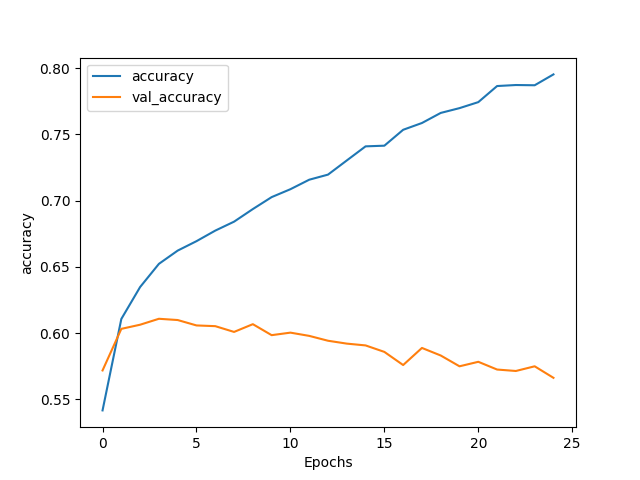
\includegraphics[scale=1.5]{img/Accuracy 2020-05_nofilter}
	\caption{Gráfica representativa del porcentaje de acierto del algoritmo, antes de aplicársele alguna mejora}
	
\end{figure}

\section{Estado de arte}

En la actualidad existen muchos algoritmos complejos de análisis de sentimientos que funcionan sin necesidad de introducirle tantos datos, tales como GPT-3 (Generative Pre-trained Transformer 3). En donde gracias a su uso eficiente de transformadores y también gracias a que ha sido entrenado extensamente con datasets enormes (por ejemplo: Wikipedia Corpus, Common Crawl, WebText2, entre otros), no hay necesidad de encontrar datos tan especificos para entrenarlos \citep{gpt3}.

La gran diferencia entre el algoritmo propuesto en este proyecto y algo más elaborado como lo es GPT-3, es el hecho de que este último no funciona localmente, sino que en realidad es una API por la cual tienes que pagar para poder usar, además de que OpenAI tiene completo control y regulación de los usos de su algoritmo \citep{openai}. 

Lo que se intenta hacer al momento de utilizar TensorFlow es darle el control completo al usuario en caso de que quiera darle sesgo a los datos o que lo adapte a las necesidades que tenga, sin necesidad de que pase a ser una caja negra. Éste proceso es bastente complicado y probablemente no se alcanzará el grado de porcentaje de acierto con el que cuenta GPT-3, pero se espera que sea lo suficiente como para poder ser una alternativa open-source viable.

\section{Solución propuesta}
La implementación se hizo en Python 3.7 \citep{python}, además de otras herramientas relacionadas con redes neuronales como Tensorflow 2.0.0 \citep{tensorflow}.


\subsection{Metodología}
Se comenzó por una búsqueda de datasets, utilizandose la librería NLTK \citep{nltk} para filtrar palabras que no aportan mucho significado al texto.

Se consideró mejor un enfoque generalista debido a que las diferentes etiquetas de sentimiento a analizar no estaban distribuidas de manera uniforme; por lo que los datos se clasificaron únicamente en \textit{"Bueno"},\textit{"Neutral"} y \textit{"Malo"}.

Se utilizó un algoritmo bidireccional STM con una activación de softmax de última capa. El léxico está limitado a 5000 elementos, y el largo máximo de cualquier frase después de ser filtrada es de 30 caracteres.

Ya después de ser actualizado, el dataset utilizado cuenta con alrededor de 60,000 tweets filtrados y clasificados.

Durante la fase de entrenamiento, se utilizaron 25 epochs con un 75\% del dataset en un orden arbitrario, usando el 25\% restante como validación.

\begin{figure}
	\centering
	\captionsetup{type=figure}
	\setcounter{figure}{1}
	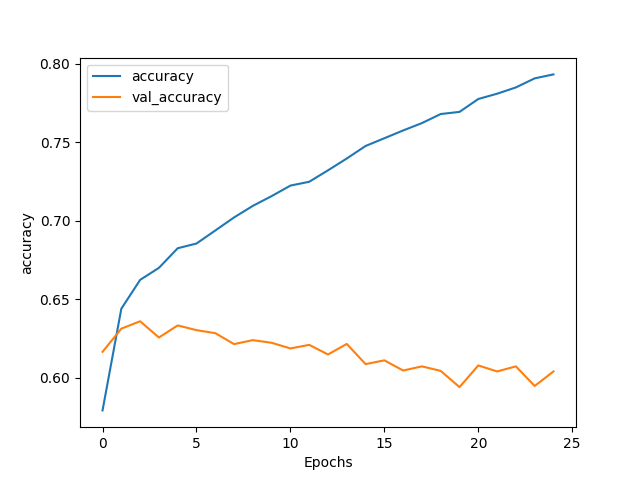
\includegraphics[scale=1.5]{img/Accuracy 2021-07.png}
	\caption{Gráfica representativa del porcentaje de acierto del algoritmo, después de aplicársele las mejoras propuestas}	
\end{figure}

\section{Experimentos}

Para determinar que este enfoque iba a funcionar, lo que hicimos fue correr varias veces el algoritmo con diferentes parámetros dentro de el, y comparando gráficas.

\begin{table}
\setcounter{table}{0} % por culpa de sciposter
\captionsetup{type=table} % por culpa de sciposter
\caption{Aquí explicas cómo interpreta el cuadro.}
\label{data}
\begin{center}
\scalebox{0.9}{\begin{tabular}{|r|c|l|}
    \hline
         \multicolumn{1}{|c|}{\rotatebox{90}{\bf Valor}}
         & \multicolumn{1}{|c|}{\rotatebox{90}{\bf Parámetro}}
         & \multicolumn{1}{|c|}{\rotatebox{90}{\bf Descripción\phantom{m}}} \\
         \hline
         0.23 & $x$ & algo \\
         \hline
         2.34 & $y$ & demo \\
        \hline
    \end{tabular}}
\end{center}
\end{table}

\section{Conclusiones}

Se ha logrado un aumento en la precisión de reconocimiento de emociones, se espera realizar más modificaciones para mejorar el algoritmo y en un futuro implementarlo para su uso.

\paragraph{Agradecimientos}

{\small Agradecemos a la dra. Elisa Schaeffer por su apoyo en la realización del póster, además de el PROVERICYT y Delfín al dar la oportunidad de participar en el Verano de Investigación Científica y Tecnológica 2021 y proporcionar una beca.
El póster se preparó con \url{https://www.overleaf.com/}.}


\bibliography{poster}
\bibliographystyle{plainnat}

\end{multicols}

\end{document}
